\documentclass[a4paper,12pt]{report}

% Chapter-style literature review prepared for an HKUST Overleaf workflow.

\usepackage[margin=1in]{geometry}
\usepackage{amsmath}
\usepackage{setspace}
\usepackage{fancyhdr}
\usepackage{titlesec}
\usepackage{booktabs}
\usepackage{longtable}
\usepackage{array}
\usepackage{float}
\usepackage{graphicx}
\usepackage{caption}
\usepackage{hyperref}
\usepackage[numbers,sort&compress]{natbib}
\hypersetup{hidelinks}

\setstretch{1.22}
\setlength{\emergencystretch}{3em}
\renewcommand{\arraystretch}{1.18}
\pagestyle{fancy}
\fancyhf{}
\fancyhead[L]{\nouppercase{\leftmark}}
\fancyhead[R]{\thepage}
\titleformat{\chapter}[display]{\bfseries\Large}{Chapter \thechapter}{0.4em}{\LARGE}
\titleformat{\section}{\large\bfseries}{\thesection}{0.8em}{}
\titleformat{\subsection}{\normalsize\bfseries}{\thesubsection}{0.8em}{}
\titlespacing*{\chapter}{0pt}{-0.5em}{1.2em}

\title{\vspace{1.5cm}\textbf{\LARGE Thermodiffusion and Thermogalvanic Effects in Ionic Thermoelectrics}\\
\vspace{0.8cm}
\large Literature Review and Research Chapters}
\author{Your Name\\
The Hong Kong University of Science and Technology}
\date{\today}

\begin{document}
\maketitle
\thispagestyle{empty}
\newpage
\tableofcontents
\newpage

\chapter{Literature Review}

This chapter examines ionic thermoelectrics through a deliberately restricted
scope. It focuses on thermodiffusion (TD) and thermogalvanic (TG) conversion in
liquid and quasi-solid electrolytes, with particular attention to TG redox
chemistry, solvent and additive effects, and polymer-gel matrices. Ion-insertion
thermoelectrochemical cycles and mixed ionic--electronic conductors are noted
only where they clarify a performance metric or a device boundary. Rather than
ranking materials by thermopower alone, the chapter follows a cross-scale
organizing principle: molecular entropy and association set the available
thermovoltage; mesoscale transport and interfaces determine how much of that
voltage survives under load; and device architecture determines whether the
output is continuous, cyclic, and practically recoverable
\citep{jabeen2024recent,kim2026functional,shang2026pushing,xu2026birdseye}.
Accordingly, the discussion proceeds from low-grade heat and thermoelectric
materials to TG solvation-entropy differences, redox couples, solvent and
additive regulation, hydrogel matrices, and the remaining research gaps.

\section{Low-Grade Heat and Thermoelectric Materials}

Low-grade heat is widely distributed in environments where the temperature is
too low for efficient recovery by conventional heat engines. It appears in
industrial warm streams, data centers, microelectronics, building surfaces, and
the human body. The relevant temperature difference is often only a few to
several tens of kelvin, so an energy-conversion technology must operate under a
small thermodynamic driving force, tolerate large areas or soft contact, and
remain inexpensive enough for distributed deployment \citep{duan2021liquid,
liu2021wearable,shang2026pushing}.

Electronic thermoelectric generators convert a temperature difference directly
into voltage through the Seebeck effect. Their solid-state operation is compact
and continuous, but high-performance electronic thermoelectric materials are
often inorganic, rigid, and optimized for temperature regimes or module formats
that are not ideal for near-room-temperature, flexible heat harvesting. More
importantly, many electronic thermoelectrics generate Seebeck
coefficients on the order of $10^2\ \mu$V K$^{-1}$, whereas ionic
thermoelectric systems can readily reach mV K$^{-1}$ thermopowers because
ions, solvent shells, and redox reactions carry much larger entropy changes
\citep{duan2021liquid,jabeen2024recent,kim2026functional}.

\begin{figure}[H]
\centering
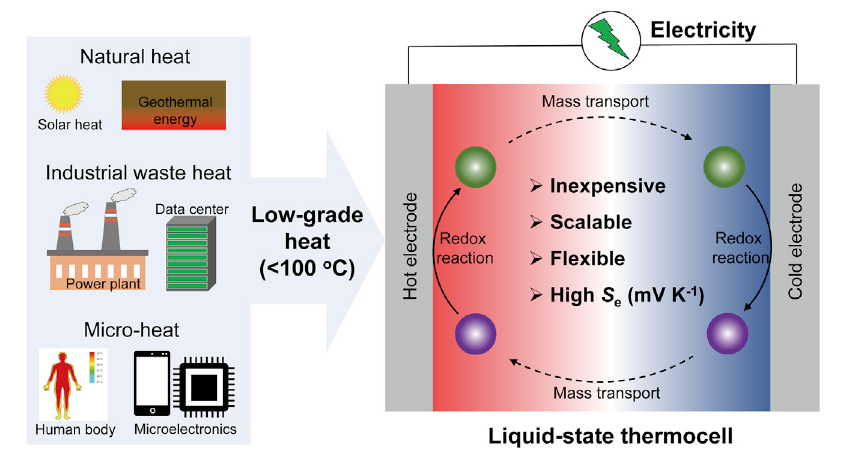
\includegraphics[width=0.9\linewidth]{figures/joule_low_grade_sources.png}
\caption{Low-grade heat sources and the liquid-state thermocell concept,
adapted from Duan et al. \citep{duan2021liquid}.}
\end{figure}

In electrolyte-based thermoelectrics, temperature gradients are converted into
electrical signals mainly through ion redistribution or redox-potential shifts.
Thermodiffusion (TD) describes the Soret-driven migration of cations and
anions, which can generate large thermovoltages through interfacial charge
accumulation. Thermogalvanic (TG) conversion instead relies on the temperature
dependence of redox equilibria at two electrodes, allowing current to be
sustained when redox mass transport and electrode kinetics remain reversible.
Mechanisms based on ion insertion, thermal extraction, or mixed ionic-electronic
transport are not discussed further because they involve distinct electrode
reactions and device architectures. The relevant contrast is therefore between
TD systems, which often exhibit large but capacitor-like outputs, and TG
systems, which provide a redox-based route to continuous heat-to-electricity
conversion.

\subsection{Historical Development}

The development of ionic thermoelectrics can be read as a gradual broadening of
what is considered an active thermoelectric material. Early thermoelectrics
focused on electronic carriers in solids. The ionic thermoelectric literature
then shifted attention to electrolytes, where temperature gradients affect ion
distributions, solvation structures, redox potentials, and electrochemical
interfaces. This shift made soft devices possible, but it also made the field
more chemically complex: the measured voltage may contain contributions from
thermodiffusion, redox entropy, concentration gradients, electrode kinetics, and
polymer-ion interactions.

\begin{figure}[H]
\centering
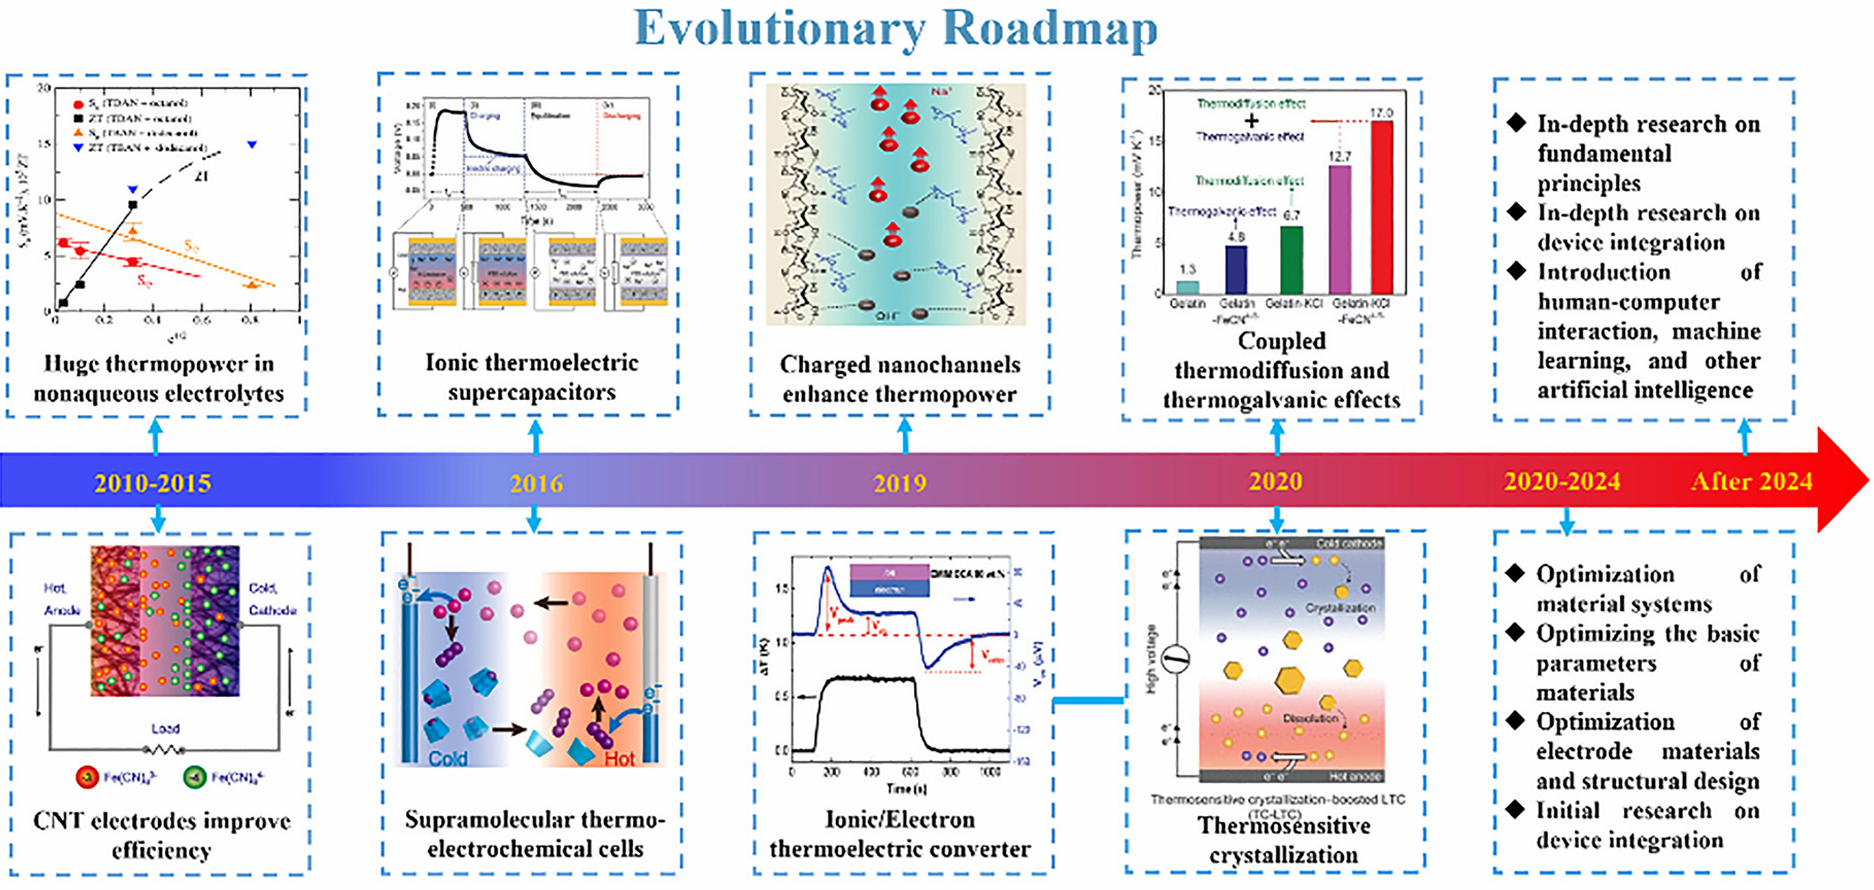
\includegraphics[width=\linewidth]{figures/csr_roadmap_full_uploaded.png}
\caption{Representative evolutionary roadmap of ionic thermoelectrics, adapted
from Shang et al. \citep{shang2026pushing}.}
\end{figure}

The roadmap in Figure 1.2 separates several stages of development.
From 2010 to 2015, nonaqueous electrolytes and nanostructured electrodes showed
that thermogalvanic systems could be improved by chemistry and interface
engineering. Around 2016, thermally charged ionic capacitors clarified how ion
redistribution can produce large thermovoltages. By 2019 and 2020,
TD--TG-coupled systems and thermosensitive crystallization showed that high
thermopower can be generated not only by choosing a redox couple, but also by
constructing spatial gradients and selective molecular interactions. Recent
reviews therefore frame TG development around redox thermodynamics,
solvation-structure control, gel electrolyte design, device integration, and
data-assisted materials design \citep{shang2026pushing}.

This development establishes a mechanism-based order for electrolyte
thermoelectrics. TD provides the high-voltage case for ion redistribution,
whereas TG defines a redox-entropy problem in which redox couples, solvation
environments, additives, and gel matrices jointly control thermopower.

\subsection{Thermodiffusion and Thermogalvanic Conversion}

\begin{figure}[H]
\centering
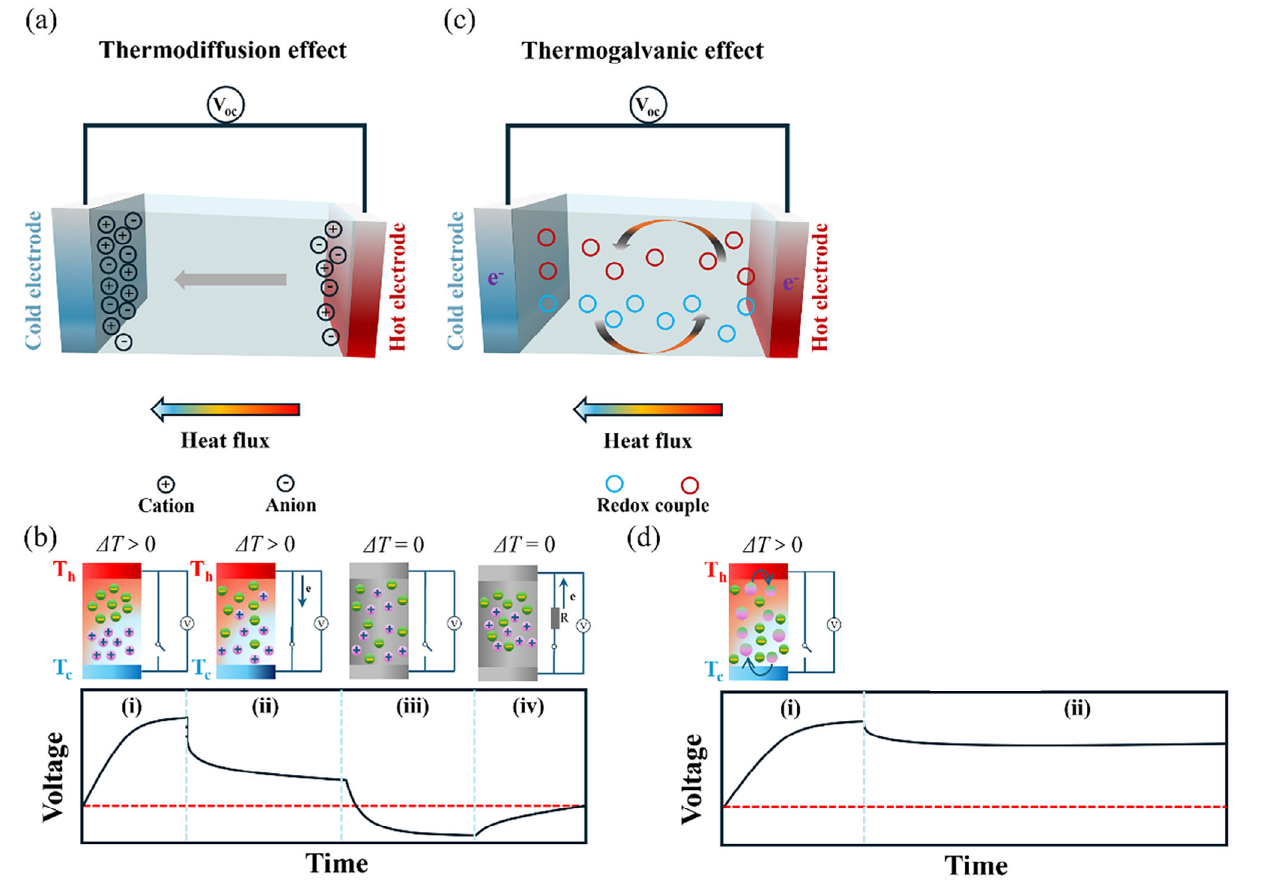
\includegraphics[width=\linewidth]{figures/as_td_tg_mechanisms.png}
\caption{Mechanistic distinction between thermodiffusion and thermogalvanic
effects in ionic thermoelectric devices, adapted from Lin et al.
\citep{lin2025critical}.}
\end{figure}

Thermodiffusion originates from the Soret effect. Under a temperature gradient,
cations and anions can migrate with different thermodiffusion coefficients.
This asymmetric ion redistribution generates concentration polarization and an
electric double layer near blocking electrodes. Thermally charged capacitors
use this effect through a cycle of voltage buildup, charging, equilibration,
and discharge. They can produce very large apparent ionic Seebeck coefficients,
but the practical output is commonly tied to charge-discharge operation and is
therefore intermittent \citep{han2020gelatin}.

Thermogalvanic cells operate differently. A redox couple is present in the
electrolyte, and the two identical electrodes are held at different
temperatures. Because the redox potential depends on temperature, the hot and
cold electrodes acquire different equilibrium potentials. Once the cell is
connected to an external circuit, oxidation and reduction occur in opposite
directions at the two electrodes, while redox ions migrate through the
electrolyte and are regenerated. This reversible redox cycle allows continuous
current generation as long as the temperature gradient, electrode kinetics, and
redox mass transport are maintained \citep{duan2018aqueous}.

\begin{table}[H]
\centering
\caption{Practical distinction between thermodiffusion-dominated and
thermogalvanic ionic thermoelectrics.}
\footnotesize
\begin{tabular}{>{\raggedright\arraybackslash}p{0.22\linewidth}
>{\raggedright\arraybackslash}p{0.34\linewidth}
>{\raggedright\arraybackslash}p{0.34\linewidth}}
\toprule
Aspect & Thermodiffusion-dominated systems & Thermogalvanic systems \\
\midrule
Primary carrier process & Cation/anion migration under a temperature gradient
and ion accumulation near blocking interfaces & Temperature-dependent redox
reaction at electrodes, coupled with redox-ion diffusion in the electrolyte \\
Device expression & Thermally charged capacitors and ionic thermoelectric
capacitors & Thermoelectrochemical cells, also called thermogalvanic cells \\
Main advantage & Very high ionic Seebeck coefficient is possible because ions
have large Eastman entropy of transfer & Continuous output is possible because
redox species are reversibly consumed and regenerated \\
Main limitation & Output often decays after connection to a load and requires a
charging/discharging sequence & Voltage is lower than many thermodiffusion
gels, and performance depends strongly on redox kinetics and mass transport \\
Representative design question & How to maximize asymmetric ion migration and
preserve the ion gradient & How to enlarge redox entropy while preserving
reversibility, solubility, and diffusion \\
\bottomrule
\end{tabular}
\end{table}

The practical distinction is therefore not only the sign or magnitude of the
Seebeck coefficient. It is the time structure of the output. A thermodiffusion
device can produce a large open-circuit voltage because ion migration and
electric-double-layer formation store charge at the interfaces. Once a load is
connected, however, the stored charge can be discharged and the voltage may
relax unless the system is reset or operated in a cycle. A thermogalvanic cell
also develops concentration gradients during operation, but the sustained current
is supplied by reversible redox reactions rather than by the discharge of a previously
charged interface.

This difference matters when comparing reported thermopowers. A TD-dominated
gel with $S_i$ of tens of mV K$^{-1}$ may be excellent for thermal sensing or
thermally chargeable capacitors, but it is not automatically a continuous power
source. A TG cell with a smaller $S_{\mathrm{TG}}$ can be more attractive for
steady low-grade heat harvesting because the redox couple closes the ionic
transport loop. Thermopower is therefore only the
first filter; reversibility, mass transport, solvation stability, and gel
architecture determine whether that thermopower can be converted into practical
output.

\section{Solvation Entropy Difference in Thermogalvanic Cells}

For a thermogalvanic cell, the thermopower is the voltage produced per unit
temperature difference:
\[
S_{\mathrm{TG}} =
\frac{\Delta V}{\Delta T}.
\]
For an ideal reversible redox process with $n$ transferred electrons, the
temperature coefficient of the electrode potential is linked to the entropy
change of the redox reaction:
\[
S_{\mathrm{TG}} \approx \frac{\Delta S_{\mathrm{redox}}}{nF},
\]
where $F$ is the Faraday constant. This expression is the simplest way to see
why thermogalvanic electrolytes can exceed traditional electronic Seebeck
coefficients. The voltage is not controlled only by carrier diffusion in a
solid; it is controlled by how much entropy changes when a redox species
changes oxidation state in a given solvent and ionic environment
\citep{kim2017high,chen2023solvation}.

In real electrolytes, this entropy is not an intrinsic property of the redox
center alone. Oxidized and reduced species may have different charge density,
coordination geometry, spin state, hydration shell, counterion association, and
hydrogen-bonding environment. A solvent or additive that interacts more strongly
with one redox state than the other changes the difference in local molecular
order between the two states. This is the solvation entropy difference, and it
has become one of the most important design variables for thermogalvanic
electrolytes \citep{chen2023solvation}.

\begin{figure}[H]
\centering
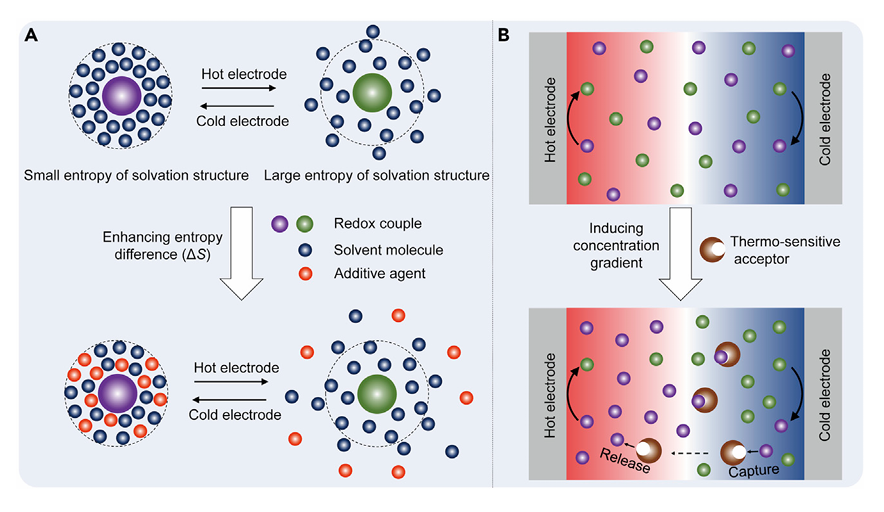
\includegraphics[width=0.92\linewidth]{figures/joule_thermopower_strategies_full.png}
\caption{Two general routes to higher thermogalvanic thermopower: increasing
the solvation-structural entropy difference and inducing a redox concentration
gradient. Adapted from Duan et al. \citep{duan2021liquid}.}
\end{figure}

The second route is concentration asymmetry. The Nernst equation indicates that
the electrode potential depends on the activity and concentration ratio of the
oxidized and reduced species. If temperature-dependent solubility,
crystallization, host-guest binding, or phase transition creates different
redox ratios at the hot and cold sides, thermopower can be amplified beyond the
baseline redox entropy contribution. This strategy is powerful but difficult:
concentration gradients are thermodynamically unstable and tend to relax by
diffusion. Recent work therefore attempts either to regenerate the gradient
continuously or to lock it into a gel, supramolecular host, or phase-separated
structure \citep{zhou2016supramolecular,yu2020thermosensitive,
guo2020nanoparticle}.

\subsection{Role of Solvation Entropy}

Solvation entropy is central because redox in a liquid is never just electron
transfer. When a species is oxidized or reduced, the solvent must reorganize to
screen the new charge distribution. If the oxidized state orders nearby solvent
molecules more strongly than the reduced state, the entropy difference between
the two states becomes large. A large entropy difference makes the redox
potential more temperature dependent, which directly increases
$S_{\mathrm{TG}}$.

This principle also explains why redox couples that look chemically similar can
perform differently in different solvents. Water, methanol, acetone, DMSO,
ethylene glycol, and deep eutectic solvents impose different hydrogen-bonding,
polarity, donor-number, and viscosity environments. These properties can change
the effective radius of the solvation shell, the activity coefficient of each
redox species, and the tendency of one redox state to crystallize or bind to an
additive. In this sense, the solvent is not a background medium; it is part of
the thermogalvanic material.

The same logic applies in polymer gels. A hydrogel contains water, polymer
functional groups, redox ions, counterions, and sometimes organic cosolvents or
fillers. Each component can change the local entropy of the redox states. A
polymer matrix that improves mechanical strength but makes both redox states
equally immobile may not improve thermopower. A matrix that selectively
stabilizes one redox state, induces a temperature-dependent concentration
profile, or maintains a hydrated transport channel can change the observed
thermogalvanic response.

\subsection{Entropy Difference and Concentration Difference}

It is helpful to distinguish two routes to larger thermopower. The first route
is an intrinsic redox-entropy route: increase the difference in entropy between
the oxidized and reduced states. This can be achieved by selecting a redox pair
with different charge density, by using a ligand environment that changes
coordination or spin state, or by using solvent/additive chemistry that
selectively reorganizes one state. The methanol-water ferri/ferrocyanide
example belongs to this route because methanol changes the solvation shell and
raises the thermopower from the aqueous baseline \citep{kim2017high}.

The second route is a concentration-gradient route. The redox potential depends
on the ratio of oxidized and reduced species. If a thermosensitive host,
crystal, gel, or phase transition changes this ratio differently at the two
electrodes, the Nernst contribution increases the voltage. The
guanidinium-induced crystallization of ferri/ferrocyanide is a representative
example: temperature-dependent crystallization and dissolution sustain a redox
concentration difference and increase thermopower to about 3.73 mV K$^{-1}$
\citep{yu2020thermosensitive}. The host-guest binding of triiodide by
$\alpha$-cyclodextrin follows the same broad idea but uses supramolecular
selectivity instead of crystallization \citep{zhou2016supramolecular}.

These two routes are not independent in practice. A guanidinium salt can change
hydration structure while also inducing crystallization. A polymer can change
redox-ion diffusion while also creating a local concentration profile. A
cosolvent can alter the entropy difference and the solubility difference at the
same time. For this reason, high thermopower should be interpreted mechanistically
rather than treated as a single number.

\subsection{From Thermopower to Recoverable Device Output}

Thermopower is an essential material descriptor, but it is not a sufficient
measure of heat-harvesting performance. The open-circuit relation
$V_{\mathrm{oc}}=S\Delta T$ states the voltage available before current is
drawn; it does not report the internal resistance, redox diffusion rate,
electrode overpotential, heat leakage, or decay of the temperature gradient.
Consequently, two cells with the same $S_{\mathrm{TG}}$ can deliver very
different power and energy. The recent reviews converge on a hierarchical
evaluation: thermopower identifies the voltage-generating chemistry;
current--voltage and impedance measurements identify kinetic losses; and
energy delivered over a defined operating period or cycle establishes whether
the chemistry is useful at the device level
\citep{duan2021liquid,jabeen2024recent,shang2026pushing,xu2026birdseye}.

For a resistive cell operated near steady state, the maximum areal power density
is commonly obtained from a load sweep, with the maximum occurring near load
matching. Normalizing this value by $(\Delta T)^2$ removes the trivial
quadratic dependence of electrical power on temperature difference, but it does
not remove dependence on electrode area, electrode spacing, orientation, or
thermal boundary conditions. Carnot-relative efficiency adds a direct
heat-to-electricity criterion, yet it remains sensitive to the hot-side
temperature and to how the heat input and effective thermal conductivity are
defined. These metrics are therefore informative only when accompanied by cell
geometry, electrode materials, temperature history, and the time at which the
measurement was taken \citep{duan2021liquid}.

The distinction between continuous TG cells and TD-dominated thermal charging
is especially important here. A peak power extracted immediately after thermal
charging can characterize a transient device, but it cannot establish sustained
power generation. For cyclic TD devices, energy delivered per complete
charge--discharge cycle and efficiency based on the corresponding thermal input
are more defensible. For TG devices intended for continuous conversion, the
relevant evidence is the stabilized current or energy delivered while a fixed
temperature difference is maintained, together with long-duration voltage and
power traces. Applying the conventional electronic
$ZT=S^2\sigma T/\kappa$ without accounting for slow ionic redistribution and
interfacial charging can therefore be misleading
\citep{jabeen2024recent,xu2026birdseye}.

\begin{table}[H]
\centering
\caption{A mechanism-aware hierarchy for evaluating ionic thermoelectric
materials and devices.}
\footnotesize
\begin{tabular}{>{\raggedright\arraybackslash}p{0.19\linewidth}
>{\raggedright\arraybackslash}p{0.25\linewidth}
>{\raggedright\arraybackslash}p{0.28\linewidth}
>{\raggedright\arraybackslash}p{0.18\linewidth}}
\toprule
Evaluation level & Recommended quantity & Question answered & Main caveat \\
\midrule
Material voltage & $S=\Delta V/\Delta T$ from multiple stabilized
$\Delta T$ values & How strongly does the material or redox environment
generate open-circuit voltage? & Does not quantify output under load \\
Transport and interface & Ionic/redox conductivity, diffusion coefficient,
impedance, and charge-transfer resistance & Which process limits current and
response time? & Values depend on electrode and geometry \\
Instantaneous device output & Full current--voltage curve and
$P_{\max}/(\Delta T)^2$ & What peak power can the stated cell deliver? &
Can overstate a decaying or cyclic output \\
Operational yield & Stabilized power and time-integrated energy, or energy per
complete cycle & How much usable electrical energy is recovered in the stated
working mode? & Requires an explicit duration or cycle definition \\
Conversion efficiency & Electrical energy divided by measured thermal input,
with Carnot-relative efficiency where appropriate & How effectively is heat
converted under the specified boundary conditions? & Sensitive to heat-loss
model and temperature definition \\
\bottomrule
\end{tabular}
\end{table}

This hierarchy changes how material strategies should be judged. Increasing
redox entropy is valuable only if the same intervention does not cause severe
ion pairing, precipitation, viscosity growth, or slow electrode kinetics.
Likewise, a gel that suppresses convection may preserve a larger temperature
difference, but its net benefit depends on whether redox transport remains fast
enough under load. The appropriate optimization target is thus recoverable
energy under a declared operating mode, not the largest isolated thermopower.

\section{Redox Couples}

The redox couple determines the sign, magnitude, and reversibility of a TG
response. Inorganic and metal-complex redox pairs are widely investigated
because they offer reversible electrochemistry, high solubility, and relatively
simple electrolyte preparation. Organic redox couples have attracted increasing
attention because proton-coupled electron transfer and phase-transition
chemistry can introduce additional entropy changes. The redox chemistry is
therefore organized below according to the origin of the entropy difference,
rather than by publication year.

\subsection{Ferri/Ferrocyanide Redox Couple}

The ferri/ferrocyanide couple, $[\mathrm{Fe(CN)}_6]^{3-/4-}$, is one of the
most widely used p-type redox couples in aqueous TG cells. Its use is supported
by reversible electrochemistry, good water solubility, and well-established
electrode kinetics. Its aqueous thermopower is commonly around 1.4 mV K$^{-1}$,
which is already large compared with electronic thermoelectric coefficients
\citep{duan2018aqueous}.

The continuing use of ferri/ferrocyanide also reflects its sensitivity to the
surrounding electrolyte environment. Methanol changes the solvation shell and
raises the thermopower. Guanidinium and urea perturb hydration shells.
Guanidinium chloride can induce thermosensitive crystallization of the
ferrocyanide-rich phase, creating a concentration difference. Gel matrices can
immobilize the liquid while preserving redox diffusion. These variations make
ferri/ferrocyanide a model system for examining how solvation, additives, and
soft matrices affect redox entropy.

\subsection{Iron Aqua Complexes and Counterion Sensitivity}

The Fe$^{2+}$/Fe$^{3+}$ system has a simpler coordination picture than
ferri/ferrocyanide, but it is more sensitive to pH, hydrolysis, and counterion
chemistry. The oxidized and reduced aqua complexes have different charge
density and hydration structures, so the entropy difference can be tuned by
changing the anion and solvent. Fe$^{2+}$/Fe$^{3+}$ is therefore relevant for
studying solvation effects, but it also makes the system more difficult to
standardize across laboratories.

Solvent-donor-number studies illustrate this sensitivity. Solvents such as
DMSO and tetramethylene sulfone change the first solvation shell around iron
ions and therefore alter the thermopower. This type of work shifts the field
from empirical additive screening toward molecular descriptors for solvation
entropy \citep{chen2023solvation}.

\subsection{Iodide/Triiodide and Supramolecular Selectivity}

The iodide/triiodide couple is frequently treated as an n-type counterpart to
ferri/ferrocyanide. Its baseline thermopower is lower than many optimized
ferri/ferrocyanide systems, but its chemistry is unusually responsive to
selective binding. Iodide is comparatively hydrophilic, whereas triiodide is
more polarizable and can interact with hydrophobic cavities or polymer domains.
This difference makes the system suitable for host-guest regulation.

The $\alpha$-cyclodextrin case illustrates the principle. Cyclodextrin can
selectively bind triiodide and create a temperature-dependent concentration
asymmetry. The thermopower increases from the baseline iodide/triiodide value
to about 1.97 mV K$^{-1}$ \citep{zhou2016supramolecular}. The mechanism is
notable because it does not rely on changing the redox couple itself. It
uses supramolecular chemistry to change the distribution of one redox state.

\subsection{Metal-Complex and Organic Redox Couples}

Metal-complex redox couples such as cobalt bipyridyl complexes are attractive
because ligands can tune charge distribution, spin state, solubility, and
electrochemical reversibility. Their main limitation is transport: ionic
liquid and deep eutectic solvent environments can give stable operation, but
high viscosity often lowers diffusion and power density. The choline
chloride-ethylene glycol deep eutectic solvent example shows that solvent
chemistry can expand the usable temperature window while keeping a measurable
thermogalvanic response \citep{antariksa2021deep}.

Organic redox couples are a newer direction. Quinone/hydroquinone derivatives,
methyl viologen, and pyrazine-based molecules are attractive because molecular
structure can be deliberately tuned. Some organic redox systems also involve
proton-coupled electron transfer, where electron transfer is coupled to proton
release or uptake. This coupling can create large entropy changes, especially
near a pH or phase transition. The hydrogel-nanoparticle thermocell based on
volume phase transition is an example of using a soft phase transition to
amplify the redox thermopower \citep{guo2020nanoparticle}.

\begin{longtable}{>{\raggedright\arraybackslash}p{0.19\linewidth}
>{\raggedright\arraybackslash}p{0.17\linewidth}
>{\raggedright\arraybackslash}p{0.32\linewidth}
>{\raggedright\arraybackslash}p{0.18\linewidth}}
\caption{Representative redox couples and reported thermopowers. Each row uses
one main source for the specific value or example.}\\
\toprule
Redox couple & Representative thermopower & Main chemical origin or design
logic & Main source \\
\midrule
\endfirsthead
\toprule
Redox couple & Representative thermopower & Main chemical origin or design
logic & Main source \\
\midrule
\endhead
$[\mathrm{Fe(CN)}_6]^{4-/3-}$ in water & about 1.4 mV K$^{-1}$ & Stable
outer-sphere redox pair; large charge difference and strong hydration make it a
widely used p-type aqueous system & \citep{duan2018aqueous} \\
$[\mathrm{Fe(CN)}_6]^{4-/3-}$ with methanol-water solvent & about 2.9 mV
K$^{-1}$ & Selective solvation-shell rearrangement of the reduced species
increases redox solvation entropy difference & \citep{kim2017high} \\
$[\mathrm{Fe(CN)}_6]^{4-/3-}$ with guanidinium/urea & about 4.2 mV K$^{-1}$
& Chaotropic and hydrogen-bonding interactions reorganize hydration structures
around ferri/ferrocyanide & \citep{duan2018aqueous} \\
$[\mathrm{Fe(CN)}_6]^{4-/3-}$ with thermosensitive crystallization & about
3.73 mV K$^{-1}$ & Guanidinium-induced crystallization and dissolution create
a redox concentration difference between electrodes & \citep{yu2020thermosensitive} \\
$\mathrm{I}^{-}/\mathrm{I}_3^{-}$ with $\alpha$-cyclodextrin & about 1.97
mV K$^{-1}$ & Host-guest binding of triiodide creates a temperature-dependent
concentration gradient & \citep{zhou2016supramolecular} \\
$\mathrm{Fe}^{2+/3+}$ in solvent-engineered electrolytes & up to several mV
K$^{-1}$ depending on solvent & Solvent donor number and hydration-shell
structure tune the entropy difference between ferric and ferrous states &
\citep{chen2023solvation} \\
$[\mathrm{Co(bpy)}_3]^{2+/3+}$ in deep eutectic solvent & about 1.67 mV
K$^{-1}$ & Coordination redox chemistry in a hydrogen-bond-rich solvent
environment & \citep{antariksa2021deep} \\
Quinone-based organic systems & about 6.7 mV K$^{-1}$ in a phase-transition
thermocell & Proton-coupled electron transfer and hydrogel nanoparticle phase
transition create a large entropy response &
\citep{guo2020nanoparticle} \\
Pyrazine-based organic redox species & above 3 mV K$^{-1}$ & Molecular redox
structure can be tuned without relying on metal complexes & \citep{lee2025pyrazine} \\
\bottomrule
\end{longtable}

Table 2 indicates a shift in design emphasis. Early work mainly treated the
redox couple as a fixed electrolyte component. Recent studies increasingly
consider the redox couple and its environment together. Ferri/ferrocyanide, for
example, has been used to examine counterion binding, methanol-water solvation,
guanidinium-induced crystallization, polymer confinement, and gel mechanics.

\section{Solvents and Additives}

The redox entropy in a TG electrolyte is determined by the redox species and
the molecular environment that reorganizes during electron transfer. Two levels
of environmental control should be distinguished. Solvent engineering changes
the continuous liquid phase in which the redox couple is dissolved. It therefore
acts broadly on dielectric screening, donor and acceptor ability,
hydrogen-bond structure, viscosity, redox solubility, and electrochemical
stability. Additive engineering introduces a secondary component selected for a
more specific interaction, such as preferential binding, chaotropic
hydration-shell disruption, counterion pairing, thermosensitive crystallization,
host--guest recognition, or polymer-chain association.

The distinction is mechanistic rather than only compositional. A water-alcohol
mixture is treated as solvent engineering when the added alcohol changes the
bulk solvation environment and transport properties. Guanidinium salts,
cyclodextrins, betaine, or crosslinking agents are treated as additives when
their main role is selective interaction with one redox state, one counterion,
or the gel network. Mixed cases exist, especially in deep eutectic solvents,
high-loading cosolvent systems, and hydrogels, but the classification should be
based on the dominant thermodynamic role rather than the ingredient name.

Thermopower can be increased either by increasing the solvation-structural
entropy difference, $\Delta S$, or by establishing a redox concentration-ratio
difference, $\Delta C_r$. This distinction provides a
mechanistic basis for grouping the later literature. Methanol-water ferri/ferrocyanide electrolytes
are a mainly solvation-entropy example \citep{kim2017high}. Guanidinium-induced crystallization is
a concentration-ratio example. Cyclodextrin-triiodide chemistry is a
host-guest concentration-ratio example \citep{yu2020thermosensitive,
zhou2016supramolecular}. Donor-number tuning of Fe$^{2+/3+}$ is
a first-solvation-shell example \citep{chen2023solvation}. Deep eutectic solvents and ionic liquids are
broader solvent-system examples, because they change volatility,
electrochemical window, ion association, and diffusion at the same time.

From the application side, solvent design also determines whether a TG cell can
operate beyond a narrow laboratory window. Water gives high ion mobility and
simple electrochemistry, but it evaporates, freezes, boils, and can trigger
side reactions at high voltage. Organic cosolvents and cryoprotectants can
extend low-temperature operation, but they may increase viscosity or reduce
biocompatibility. Ionic liquids and deep eutectic solvents reduce volatility
and broaden temperature range, but they often introduce stronger ion-ion
correlation and slower diffusion. Thus, solvent engineering is not a simple
route to a larger $S_{\mathrm{TG}}$; it is a four-way compromise among
thermopower, solubility, conductivity, and stability.

\begin{figure}[p]
\centering
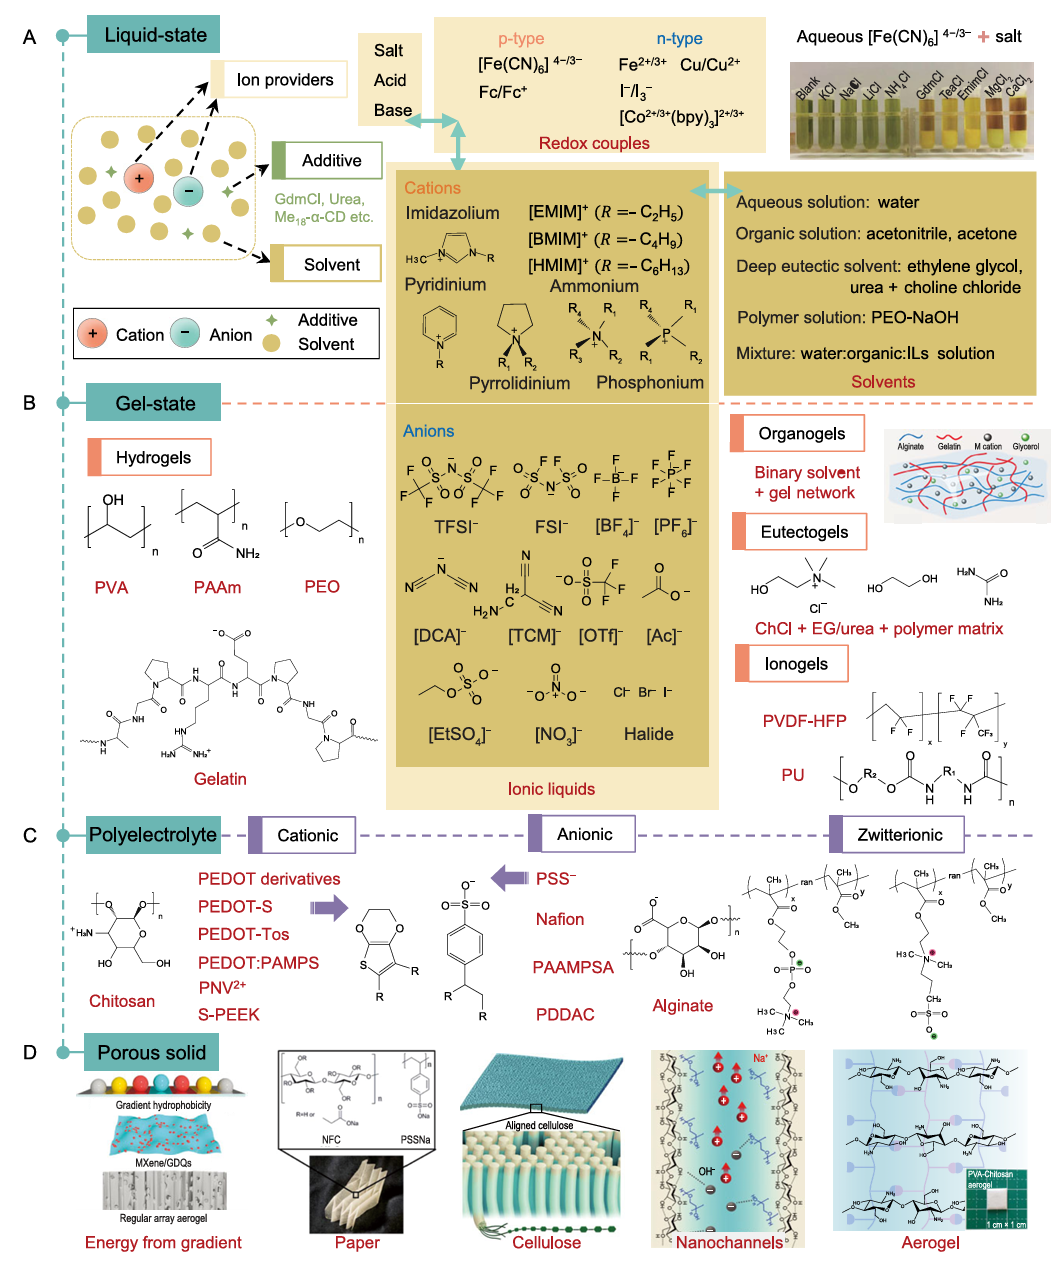
\includegraphics[width=\linewidth,height=0.84\textheight,keepaspectratio]
{figures/nsr_material_categories_full.png}
\caption{Material classes and representative constituents of ionic
thermoelectrics, spanning liquid-state electrolytes, gel-state electrolytes,
polyelectrolytes, and porous solids. Adapted from Xu et al.
\citep{xu2026birdseye}.}
\end{figure}

Table 3 separates bulk-solvent strategies from additive strategies. The former
modify the continuous electrolyte environment, whereas the latter rely on a
specific molecular or ionic interaction superimposed on that environment. This
separation is necessary because similar thermopower values can arise from
different physical origins: solvent-shell reorganization, temperature-dependent
solubility, selective binding, crystallization, or polymer-network effects.

\begin{longtable}{>{\raggedright\arraybackslash}p{0.18\linewidth}
>{\raggedright\arraybackslash}p{0.17\linewidth}
>{\raggedright\arraybackslash}p{0.31\linewidth}
>{\raggedright\arraybackslash}p{0.19\linewidth}}
\caption{Representative solvent and additive strategies. Solvent rows refer to
changes in the bulk liquid phase; additive rows refer to selective molecular,
ionic, or polymer-network interactions.}\\
\toprule
Redox pair & Component & Main role & Source \\
\midrule
\endfirsthead
\toprule
Redox pair & Component & Main role & Source \\
\midrule
\endhead
$[\mathrm{Fe(CN)}_6]^{4-/3-}$ & Solvent: methanol-water mixture & Rearranges the
solvation shell and increases the redox solvation entropy difference; the
reported thermopower rises to about 2.9 mV K$^{-1}$ & \citep{kim2017high} \\
$[\mathrm{Fe(CN)}_6]^{4-/3-}$ & Additives: guanidinium and urea & Perturbs hydration
shells through chaotropic and hydrogen-bonding effects; the reported
thermopower reaches about 4.2 mV K$^{-1}$ & \citep{duan2018aqueous} \\
$[\mathrm{Fe(CN)}_6]^{4-/3-}$ & Additive: guanidinium chloride & Induces
thermosensitive crystallization/dissolution of $[\mathrm{Fe(CN)}_6]^{4-}$ and
creates a redox concentration difference & \citep{yu2020thermosensitive} \\
$\mathrm{I}^{-}/\mathrm{I}_3^{-}$ & Additive: $\alpha$-cyclodextrin & Selectively binds
triiodide and establishes a temperature-dependent concentration gradient &
\citep{zhou2016supramolecular} \\
$\mathrm{Fe}^{2+/3+}$ & Solvents with different donor numbers &
Changes the first solvation shell and the entropy difference between
Fe$^{3+}$ and Fe$^{2+}$ & \citep{chen2023solvation} \\
$[\mathrm{Co(bpy)}_3]^{2+/3+}$ & Solvent: ChCl-EG deep eutectic solvent & Provides a
low-volatility hydrogen-bonding solvent network
for thermogalvanic operation at middle temperature & \citep{antariksa2021deep} \\
Quinone redox system & Gel NPs & Uses volume
phase transition and pH-sensitive PCET chemistry to amplify the thermal
response & \citep{guo2020nanoparticle} \\
\bottomrule
\end{longtable}

The common theme is that solvent and additive design must be judged by two
entropy terms rather than by a single ingredient name. One term is the
solvation-structural entropy difference between redox states. The other is the
concentration-ratio contribution that appears when the oxidized and reduced
species are not distributed identically at the hot and cold electrodes. The
most successful designs often use both: guanidinium chemistry modifies
ferri/ferrocyanide solvation while also enabling thermosensitive
crystallization, and cyclodextrin chemistry increases the effective
concentration asymmetry of triiodide through selective host-guest binding.

\subsection{Solvent Engineering}

Solvent engineering acts on three properties at once. The first is redox
entropy, because the solvent shell reorganizes during electron transfer. The
second is solubility, because the oxidized and reduced species may have
different temperature-dependent solubilities. The third is transport, because
viscosity controls how fast redox ions can diffuse between the electrodes.
Good solvent design therefore requires a compromise: the solvent must make the
redox states entropically different, but it must not immobilize the ions so
strongly that current output collapses.

Methanol-water ferri/ferrocyanide electrolytes illustrate a relatively clean
solvation effect. The redox couple is unchanged, but the local solvent
environment changes enough to increase thermopower. This provides a clear
mechanistic control: thermogalvanic thermopower can be modified
without introducing a new redox molecule \citep{kim2017high}.

The methanol case also clarifies what is meant by "solvent engineering." The
added alcohol does not simply dilute the aqueous electrolyte. It changes the
relative organization of solvent molecules around the two charge states of the
redox pair. Because $[\mathrm{Fe(CN)}_6]^{4-}$ has a larger charge magnitude
than $[\mathrm{Fe(CN)}_6]^{3-}$, it is more sensitive to changes in the
hydrogen-bonding environment. The thermopower increase from about 1.4 to
2.9 mV K$^{-1}$ therefore comes from making the solvation entropy difference
between the reduced and oxidized species larger. The mechanistic implication is
that a widely used redox couple can be treated as a solvent-responsive
thermodynamic unit rather than as a fixed electrolyte component.

Organic cosolvents can also work through solubility and temperature-dependent
phase behavior rather than through a purely local solvation shell. A
bacterial-cellulose hydrogel containing ferri/ferrocyanide
in a water/propylene glycol medium, where propylene glycol promotes gradual
crystallization of $K_4[\mathrm{Fe(CN)}_6]$ and thereby introduces a redox
concentration contribution to thermopower \citep{yin2023bacterial}. In that
case, spectroscopic evidence suggested that the cyano ligand environment did
not change strongly; the performance increase was instead assigned mainly to
the concentration-ratio term. Ethylene glycol in PAAm-based ferri/ferrocyanide
hydrogels provides another example of solvent design serving a device-level
function: it suppresses freezing by disturbing the water hydrogen-bond network,
while the different solubility of ferricyanide and ferrocyanide helps generate
a thermally dependent redox distribution \citep{liu2024subzero}. These cases
show why "cosolvent" should not be treated as a single mechanism. It may tune
solvation entropy, crystallization, freezing resistance, or several of these
simultaneously.

For Fe$^{2+/3+}$ electrolytes, donor-number control provides a more direct
connection between solvent coordination and thermopower. Solvents with
different donor numbers can stabilize Fe$^{3+}$ and Fe$^{2+}$ to different
degrees, changing the structure and disorder of the first solvation shell. The
PAAm/water Fe$^{2+/3+}$ system shows that a
high-donor-number solvent reduced the ionic Seebeck coefficient, whereas a
lower-donor-number solvent raised it to about 2.49 mV K$^{-1}$
\citep{chen2023solvation}. Free-energy
perturbation and molecular-dynamics calculations for water/acetone systems,
where high acetone fraction was associated with a more ordered solvation shell
and larger thermopower \citep{chen2023solvation}. These studies matter because
they move the field beyond empirical solvent screening: the target becomes the
relative solvation entropy of the two redox states, which can in principle be
predicted.

Deep eutectic solvents show a different balance. They are less volatile than
water-rich electrolytes and can operate over broader temperature windows, but
their viscosity can restrict ion diffusion. Their value is therefore not only
high thermopower; it is the ability to combine redox entropy modulation with
practical stability. This is especially relevant for devices that must operate
outside a narrow ambient-temperature window \citep{antariksa2021deep}.

The IL and DES literature should be read in this practical context. Ionic
liquids provide nonvolatile and thermally stable media when water evaporation
or boiling would restrict operation, although their higher viscosity can reduce
redox diffusion and power output \citep{russo2019hydrogels}. A representative DES example is the
$[\mathrm{Co(bpy)}_3]^{2+/3+}$ thermocell in choline
chloride/ethylene glycol, where a hydrogen-bond-rich, low-volatility solvent
network supported middle-temperature operation with a thermopower of about
1.67 mV K$^{-1}$ \citep{antariksa2021deep}. Water-containing DES gels then add
another layer: the DES adjusts redox solvation and freezing resistance, while
the gel network supplies dimensional stability.

Counterion and ligand effects are closely related to solvent effects, because
they determine how tightly the redox center is paired or coordinated. In
Fe$^{2+/3+}$ systems, weakly coordinating anions such as perchlorate can reduce
ion pairing and stabilize aquo complexes, producing higher thermopower and
better effective conductivity than more strongly interacting counterions
\citep{duan2018aqueous}. Ligand design plays an analogous role in metal-complex
redox couples. Introducing ethylenediamine ligands into copper complexes, for
example, changes the coordination environment and reaction entropy, illustrating
that the solvent shell and the primary coordination sphere should be considered
together. These cases sit
between "redox-couple selection" and "solvent selection": the redox formula
changes, but the performance gain is still largely environmental and entropic.

\subsection{Additives as Local Entropy Modifiers}

Additives are attractive because they can be introduced at low concentration
and targeted toward one interaction. Guanidinium chemistry is the clearest
example in ferri/ferrocyanide systems. In one case, guanidinium and urea
change the hydration shell and increase the redox solvation entropy difference
\citep{duan2018aqueous}. In another case, guanidinium chloride induces
thermosensitive crystallization, so the key effect is a concentration
difference rather than only a solvation-shell difference
\citep{yu2020thermosensitive}. These two cases should not be merged into a
single "guanidinium additive" mechanism. They use related chemistry, but the
dominant thermodynamic contribution is different.

The guanidinium/urea aqueous ferri/ferrocyanide work is best understood as a
hydration-shell design study. Guanidinium is a chaotropic cation with strong
interactions toward the highly charged ferrocyanide ion, while urea reorganizes
the surrounding hydrogen-bond network. Together they amplify the difference
between the solvation environments of $[\mathrm{Fe(CN)}_6]^{4-}$ and
$[\mathrm{Fe(CN)}_6]^{3-}$, raising the thermopower to about 4.2 mV K$^{-1}$
\citep{duan2018aqueous}. The work made the
solvation-entropy mechanism experimentally tangible: the additive was not
introduced as an inert salt, but as a molecular tool for making one redox state
more structurally distinct from the other.

The thermosensitive-crystallization work using guanidinium chloride should be
kept separate. Here the major design move is the selective formation and
dissolution of ferrocyanide-associated crystals at different temperatures. The
cold side becomes depleted or enriched in one redox species relative to the
other, so the Nernst concentration term contributes to the open-circuit
voltage. The reported thermopower of about 3.7 mV K$^{-1}$ and high
Carnot-relative efficiency come from a coupled improvement: concentration
asymmetry boosts voltage, crystal formation suppresses convection, and the
local redox ratio can favor electrode reactions \citep{yu2020thermosensitive}.
The result shows that a concentration gradient, usually assumed to relax away,
can be stabilized by temperature-dependent association.

Cyclodextrin-based additives work through a third mechanism: supramolecular
recognition. Instead of perturbing all hydration shells, cyclodextrin
selectively binds triiodide. The binding changes the free concentration of one
redox species, and the temperature dependence of that binding creates a redox
concentration gradient. This mechanism explains why host-guest chemistry has
become part of thermogalvanic design
\citep{zhou2016supramolecular}.

The same logic appears in later thermoresponsive iodine systems. PNIPAM- and
methyl-cellulose-containing electrolytes can interact selectively with
triiodide when the polymer becomes more hydrophobic above its transition
temperature, changing the local concentration of active iodine species and even
allowing apparent p/n conversion in some temperature regimes
\citep{duan2019pn}. These systems are not merely "iodide redox couples in
gels." They use the redox equilibrium, host or polymer affinity, and thermal
phase behavior as a single coupled design element. Their advantage is strong
thermal selectivity. Their limitation is that the operating temperature window is
defined by the host or polymer transition, so response reversibility and
cycling stability become as important as the absolute thermopower.

Some additives are introduced directly into hydrogels, where their function is
both thermodynamic and mechanical. In a gelatin/ferri-ferrocyanide hydrogel,
betaine acts as a zwitterionic additive that interacts
with polymer chains while selectively rearranging the solvation structure of
ferricyanide, giving a thermopower near 2.2 mV K$^{-1}$
\citep{lu2024zwitterion}. In another gel example, glutaraldehyde crosslinking in
gelatin-based systems strengthens the matrix while also interacting with
ferri/ferrocyanide, leading to a much larger reported ionic thermopower in a
coupled ionic thermoelectric material. These cases
show why hydrogel additives are harder to classify than liquid additives: the
same molecule may tune polymer chain mobility, water retention, redox
solvation, and mechanical integrity.

Filler additives add another layer of complexity. MXene-containing hydrogels can
improve mechanical strength, self-healing behavior, and interfacial contact.
However, conductive or redox-active fillers also bring
risks. They may change electron-transfer pathways, alter the local temperature
field, or make it harder to separate thermogalvanic voltage from other ionic or
electronic effects. For this reason, filler-based TG hydrogels should report
mechanical durability and power output together with controls that isolate the
redox contribution.

\subsection{Transport and Stability Trade-Offs}

Solvents and additives can improve thermopower while damaging other parts of
the device. A strong interaction can increase entropy contrast but also slow
diffusion. Crystallization can build a concentration difference but can also
cause sedimentation, orientation dependence, or long-term instability. Organic
solvents can suppress freezing but may reduce biocompatibility or change
electrode compatibility. Deep eutectic solvents can reduce volatility but may
increase viscosity. Therefore, an informative additive strategy must report not only
$S_{\mathrm{TG}}$, but also conductivity, stability, reversibility, and the
conditions under which the additive remains chemically benign.

Across the reviews, the most reliable design rule is therefore not "add a
chaotrope" or "use an organic solvent." It is to identify the dominant
thermodynamic lever and then check the transport penalty. If the lever is
solvation entropy, the evidence should include changes in redox solvation,
ion-pairing, or coordination structure. If the lever is concentration
asymmetry, the evidence should show selective binding, crystallization, or
phase partitioning under a temperature gradient. If the lever is a
polymer-assisted effect, the evidence should distinguish redox entropy from
thermodiffusion and from mechanical improvements. Without this distinction,
different works can appear to be variations of the same additive recipe even
when the dominant thermodynamic contribution is different.

\section{Hydrogel Matrices}

Gel matrices address the most immediate weakness of liquid thermogalvanic
cells: leakage and difficult packaging. In a gel thermocell, the matrix retains
water or organic solvent, immobilizes the electrolyte shape, improves contact
with soft or curved surfaces, and allows wearable or flexible device formats.
However, a gel is not only a container. Polymer functional groups can interact
with redox ions, counterions, and solvent molecules, thereby changing
solvation, diffusion, crystallization, and mechanical stability at the same
time \citep{lin2024triple,lu2024zwitterion,yin2023bacterial}.

Gelatin illustrates the possibility of coupling thermodiffusion and
thermogalvanic contributions. A gelatin-KCl-ferri/ferrocyanide system reached
a thermopower of 17 mV K$^{-1}$, far above the baseline thermogalvanic
coefficient of ferri/ferrocyanide, because the charged gelatin network and KCl
thermodiffusion contributed strongly in addition to the redox reaction
\citep{han2020gelatin}. This system should not be confused
with a purely thermogalvanic record; it is a coupled ionic thermoelectric
system.

Poly(vinyl alcohol) (PVA), polyacrylamide (PAAm), bacterial cellulose, and
double-network hydrogels represent the main polymer directions in
thermogalvanic gels. PVA offers simple processing, hydroxyl-rich hydration, and
mechanically trainable networks. PAAm provides high water content and can be
combined with ionic or covalent crosslinks for toughness. Bacterial cellulose
offers aligned nanofibrils and mechanical reinforcement. Composite gels add
cellulose nanofibers, MXene, carbon materials, or supramolecular components to
balance thermopower, ion transport, and deformation resistance
\citep{zhou2020hydrogel,yang2023strong,liu2024armor,lin2024triple}.

The design logic of gel thermogalvanic cells is therefore multiscale. At the
molecular scale, the matrix should enhance redox solvation contrast or
concentration asymmetry. At the transport scale, it should preserve redox-ion
diffusion and electrode access. At the device scale, it should maintain
hydration, temperature difference, and mechanical contact during bending,
drying, or repeated thermal cycling. This multiscale requirement explains why
recent reviews treat polymer matrices, solvent composition, additives, and
device architecture as coupled design variables rather than separate
optimization steps \citep{kim2026functional,shang2026pushing,xu2026birdseye}.

The historical development of gel TG electrolytes can be divided into three
stages. The first stage was leakage prevention: polymers were used mainly to
hold liquid electrolyte in place. The second stage was compatibility screening:
researchers asked which polymers could gel ferri/ferrocyanide or metal-complex
electrolytes without suppressing redox diffusion. The third stage is active
polymer design: the matrix is expected to tune solvation, promote selective ion
transport, regulate crystallization, and survive mechanical deformation.
Representative early studies established gel compatibility and leakage-free
operation \citep{wu2017gelled,jin2016quasisolid,russo2019hydrogels}; more recent
work treats polymer chemistry as an active handle for ion dynamics, mechanics,
and heat harvesting \citep{lin2024triple,lu2024zwitterion,liu2024subzero}.

Early ferri/ferrocyanide gels reveal why polymer compatibility cannot be
assumed. Poly(sodium acrylate) gels could maintain voltammetric behavior close
to aqueous ferri/ferrocyanide and pass simple inversion tests, suggesting that
the anionic redox species remained mobile in a quasi-solid matrix
\citep{wu2017gelled}. PVA was attractive because of its processability and
mechanical strength, but high ferri/ferrocyanide loading could cause
flocculation or reduced output in some formulations \citep{russo2019hydrogels}.
CMC and PAAm were later identified as effective hosts for higher-concentration
ferri/ferrocyanide gels, whereas some polyurethane or physically gelled systems
showed poor power output because redox transport was restricted
\citep{russo2019hydrogels}. This early screening literature is not obsolete. It
establishes a basic rule that remains valid in modern hydrogel designs: a good
matrix must be chemically compatible with the redox couple before it can be
used for more ambitious solvation or mechanical engineering.

Cellulose-based quasi-solid electrolytes introduced a different design idea.
Instead of dissolving the polymer into the electrolyte, an insoluble cellulose
network can lock the redox solution inside a porous skeleton.
Cellulose-ferri/ferrocyanide systems show that the network
provided mechanical reinforcement and a tortuous transport pathway, with an
optimized cellulose content balancing redox diffusion, mechanical integrity, and
thermal management \citep{jin2016quasisolid}. Later bacterial-cellulose and
cellulose-nanofiber systems extend this idea by using nanofibrils not simply as
passive scaffolds, but as structural elements that can form aligned pathways,
reinforce double networks, or cooperate with cosolvents and salts
\citep{yin2023bacterial,lin2024triple}. The design lesson is that a polymer matrix can control
three transport processes at once: ion diffusion, water/solvent retention, and
heat leakage.

\subsection{Gelatin Systems}

Gelatin demonstrates that biopolymer networks can
contribute actively to ionic thermoelectric behavior. The gelatin-KCl-
ferri/ferrocyanide system is often cited because it reached a very high
thermopower of 17 mV K$^{-1}$ near room temperature \citep{han2020gelatin}.
The mechanism is not purely thermogalvanic. The redox couple contributes a TG
voltage, while KCl thermodiffusion and the charged gelatin network contribute
additional ionic thermopower. Gelatin is therefore a representative case for
coupled TD-TG systems and shows why mechanism separation is required.

For thermogalvanic hydrogels, gelatin offers water retention, biocompatibility,
and functional groups that can interact with ions. Its weakness is that
mechanical stability and dehydration resistance may be insufficient without
crosslinking, additives, or encapsulation. Gelatin-based systems are therefore
best understood as a starting point for bio-derived soft thermogalvanic
materials rather than as a universal matrix.

The later gelatin literature uses this starting point in two different ways.
One route treats gelatin as a soft, ion-containing host for coupled
thermodiffusion and thermogalvanic conversion. In these systems, a large
reported ionic thermopower can originate from both the redox entropy and the
Soret response of mobile ions, so the mechanism has to be decomposed before
comparing it with a purely TG electrolyte. The other route treats gelatin as a
chemically functional scaffold. Zwitterionic or crosslinking additives can
change chain packing and water structure while also influencing redox solvation.
Gelatin systems can couple crosslinking and ferri/ferrocyanide interactions
with mechanical reinforcement and high thermopower. For a TG-focused literature review, the
central point is not the magnitude alone, but that
biopolymer-rich gels force the field to separate redox entropy, ion
thermodiffusion, water management, and network mechanics.

\subsection{PVA and PAAm Systems}

PVA and PAAm are widely used because their polymer networks are easy to tune.
PVA has hydroxyl groups that help retain water and form physically crosslinked
structures. Mechanical training or freeze-thaw processing can align polymer
domains, producing ion-transport pathways. PAAm has high water content and can
be combined with ionic crosslinks or double networks to improve toughness.

The central question for PVA and PAAm is how to improve mechanics without
blocking redox diffusion. A stiff network may suppress leakage and improve
wearability, but it can increase mass-transport resistance. A loose network may
give high ion mobility, but it may dry, deform, or leak. Thermogalvanic hydrogel
design therefore differs from ordinary hydrogel mechanics: the matrix must
remain mechanically robust while keeping the redox couple electrochemically
available.

PVA systems show why processing can be as important as composition. Hydroxyl
groups help retain water and form reversible hydrogen bonds, while freeze-thaw
or stretching treatments can create crystalline or aligned domains. PVA-based
gel strategies can also connect processing to effective conductivity:
salting-out or directional-freezing
methods can create water-rich channels and anisotropic structures that reduce
transport resistance. These examples point to a
mesoscale design principle. If the polymer-rich phase carries mechanical load
and the water-rich phase carries redox ions, the gel can be tough and conductive
at the same time.

PAAm systems are relevant because the neutral amide network can accommodate
aqueous redox species and can be combined with other networks. Early wearable
TGC studies found PAAm to be one of the more effective ferri/ferrocyanide hosts
when compared with several other gelators \citep{russo2019hydrogels}. Later work
uses PAAm as a structural framework for much more complex electrolytes.
PAAm/PVA/cellulose-nanofiber triple-network hydrogels use
PAAm for shape construction, PVA for flexibility, and cellulose
nanofibers reinforce the network; the optimized structure reached an ionic
conductivity of 168 mS cm$^{-1}$ and a reported $ZT$ of 0.06
\citep{lin2024triple}. Conductivity is therefore treated as a structural
property of the gel, not only as a concentration
property of the dissolved redox couple.

PAAm also appears in n-type Fe$^{2+/3+}$ gel systems, where the challenge is
different. Fe$^{2+/3+}$ can be soluble and chemically robust, but its
thermopower depends strongly on counterion, solvent, and coordination
environment. Non-aqueous or mixed-solvent PAAm gels can combine Fe$^{2+/3+}$
redox chemistry with anti-freezing behavior \citep{liu2024subzero}. These systems matter for device
integration because p-type ferri/ferrocyanide cells alone do not provide the
ideal p/n module architecture. High-performance n-type gels remain a bottleneck
for compact series-connected modules.

\subsection{Cellulose and Composite Gels}

Cellulose-based gels add another design route. Bacterial cellulose can provide
nanofiber reinforcement and internal channels. Cellulose nanofibers can be
combined with synthetic networks to improve toughness and dimensional stability.
Composite gels can also include MXene, carbon materials, or conductive
polymers, but these fillers must be used carefully. They can improve mechanical
properties or electrode contact, yet they can also change interfacial reactions
or introduce parasitic pathways.

The thermogalvanic hydrogel literature therefore increasingly emphasizes
multiscale design. At the molecular scale, polymer functional groups and
cosolvents tune solvation entropy. At the mesoscale, phase separation,
nanofibers, and aligned channels control ion transport. At the device scale,
encapsulation, electrode contact, and module geometry determine whether the
temperature gradient and redox flux are maintained. A hydrogel is successful
only when these scales are compatible.

Bacterial cellulose is especially attractive because it can combine mechanical
strength with aqueous channels. In water/propylene glycol ferri/ferrocyanide
systems, bacterial cellulose acts as a hydrogel scaffold while the cosolvent
controls crystallization and low-temperature stability \citep{yin2023bacterial}.
In hybrid cellulose-PAAm systems, cellulose nanofibers add reinforcement and can
help organize ion-transport pathways \citep{lin2024triple}.
A large thermopower does not lead to high power output if the redox species
cannot move fast enough to support current under load.

Composite fillers such as MXene, carbon materials, and conductive polymers must
be interpreted carefully. In a mechanical sense, they can dissipate energy,
increase stretchability, and improve contact with electrodes. In an electrical
or electrochemical sense, they may introduce additional charge-transfer sites or
mixed ion-electron pathways. MXene-containing hydrogels can retain thermopower
under repeated deformation, demonstrating the device value of robust soft
materials. However, for mechanistic clarity, such systems should
be reported with controls that separate matrix mechanics, electrode kinetics,
and bulk TG voltage.

\subsection{Thermoresponsive and Functional Polymer Matrices}

Thermoresponsive polymers move beyond passive gelation by making the matrix
itself temperature-selective. In iodine-based systems, PNIPAM or methyl
cellulose can change hydrophobicity near a transition temperature and thereby
alter the local activity of $\mathrm{I}_3^-$ \citep{duan2019pn}. This is
conceptually similar to cyclodextrin binding, but the host is now a polymer
network whose affinity changes with temperature. The benefit is strong thermal
amplification and possible sign reversal. The drawback is that performance
depends on the phase-transition window and on whether repeated heating and
cooling preserve the same polymer morphology.

Functional side chains provide another route. Copolymer and zwitterionic
designs use cationic or sulfobetaine groups that
selectively interact with Fe$^{3+}$ or ferri/ferrocyanide ions, changing
hydration and redox entropy \citep{lu2024zwitterion}. This line of work is
relevant because it connects TG electrolytes with polymer physics: side-chain
charge, segmental mobility, hydration, and ion association are all variables
that can be designed. In a liquid electrolyte, the solvent shell is determined
mainly by small molecules. In a functional polymer electrolyte, the redox
species experiences a heterogeneous environment containing water, counterions,
polymer segments, and sometimes nanoscale phase separation.

Chitosan-based and guanidinium-containing polymer networks illustrate how
polymer chemistry can combine entropy and concentration effects. A
chitosan/guanidine/melamine double-network FeCl$_3$/FeCl$_2$ system uses
cationic groups to accelerate chloride migration and melamine to complex
Fe$^{3+}$ near the cold side, increasing both entropy and
concentration-difference contributions \citep{hu2024doubleselective}. The design
extends beyond gelation. It uses polymer functional groups,
redox-ion coordination, and thermodiffusive ion movement together. Such systems
are powerful, but they also make mechanism attribution more demanding because
TG, TD, and complexation-driven concentration gradients can all contribute to
the measured voltage.

\subsection{Gel Transport, Thermal Conductivity, and Device Stability}

Gelation suppresses natural convection, which is one reason gels can improve
effective thermal management relative to liquids. Joule 2021 emphasized that
effective thermal conductivity in liquid thermocells includes convection under a
temperature gradient, and that gel-based electrolytes can reduce this
contribution \citep{duan2021liquid}. This is a major advantage for maintaining
a usable $\Delta T$ across the electrodes. The penalty is that gels often reduce
redox diffusion. Therefore, modern hydrogel design tries to decouple thermal
and ionic transport: suppress convective heat flow while preserving continuous
aqueous or solvent-rich ion pathways.

Several strategies address this trade-off. Directional freezing can create
aligned channels. Salting-out can form polymer-rich and water-rich domains.
Nanofibers can reinforce the network without filling all transport space.
Low-eutectic or mixed-solvent systems can keep water mobile over a wider
temperature range. These are effective-conductivity strategies rather than
purely mechanical modifications.
The relevant conductivity for TG power output is not
only the small-ion conductivity measured in a homogeneous electrolyte, but the
combined resistance of redox diffusion, ion migration, polymer confinement, and
electrode reactions.

Device stability adds another set of constraints. Wearable TGCs bend, stretch,
dry, warm, cool, and repeatedly lose and regain contact with the skin or heat
source. Flexible electrodes, gel electrolytes, and stable hydrogel-electrode
interfaces must therefore be treated as parts of the same device problem.
Strong and self-healing hydrogels
extend the operating lifetime, but mechanical durability is only meaningful if
the redox couple remains reversible and the thermopower is retained after
deformation. Reports that include stretching cycles, cutting/healing cycles,
anti-freezing tests, and long-term thermal cycling are therefore more
informative than reports that only give an initial $S_{\mathrm{TG}}$.

\begin{longtable}{>{\raggedright\arraybackslash}p{0.18\linewidth}
>{\raggedright\arraybackslash}p{0.22\linewidth}
>{\raggedright\arraybackslash}p{0.33\linewidth}
>{\raggedright\arraybackslash}p{0.14\linewidth}}
\caption{Representative gel-matrix design principles for thermogalvanic
electrolytes.}\\
\toprule
Matrix type & Typical redox/electrolyte choice & Main design function & Main
source \\
\midrule
\endfirsthead
\toprule
Matrix type & Typical redox/electrolyte choice & Main design function & Main
source \\
\midrule
\endhead
Gelatin & KCl and $[\mathrm{Fe(CN)}_6]^{4-/3-}$ & Couples thermodiffusion in
the salt with thermogalvanic redox chemistry; clarifies why very
large thermopower may not be purely TG & \citep{han2020gelatin} \\
Evaporative hydrogel & $[\mathrm{Fe(CN)}_6]^{4-/3-}$ hydrogel & Combines heat
harvesting with evaporative cooling; highlights the role of water management
in soft TECs & \citep{zhou2020hydrogel} \\
Strong tough hydrogel & Thermogalvanic hydrogel network & Uses mechanical
reinforcement to improve durability while preserving thermoelectric response &
\citep{yang2023strong} \\
Flexible armor-type hydrogel & Thermogalvanic hydrogel device & Emphasizes
mechanical protection, flexibility, and high Carnot-relative efficiency for
practical form factors & \citep{liu2024armor} \\
\bottomrule
\end{longtable}

\section{Research Gap}

Solvent modification provides a direct means of changing the reaction entropy
of a redox couple, but the relation between solvent properties, solvation
structure and thermopower remains poorly resolved. Thermogalvanic measurements
are scarce and are reported for different redox couples, concentrations and
experimental conditions. The available dataset is therefore too small for
straightforward numerical regression. The problem is compounded by the
ion--ion and ion--solvent interactions that determine the local environments
of the oxidized and reduced species. These interactions cannot be described
reliably by a single solvent parameter. Previous data-driven studies of thermal
energy materials have shown the value of machine learning, but they also make
clear that a thermogalvanic model must be built around the limited data rather
than assuming a large, uniform database \citep{wu2024unlocking,li2022mlthermal}.
This motivates the use of DFT-derived ion--solvent interaction features and a
small-data learning strategy.

Hydrogels add a second level of complexity. Most work on thermogalvanic gels
has focused on thermopower, ionic conductivity, mechanical strength,
stretchability and stability \citep{yang2023strong,gao2022anisotropic}.
These properties are essential for devices, but they do not isolate the role of
the polymer in the solvation of the redox couple. The polymer network changes
water activity, solvent organization, local polarity and molecular motion.
Consequently, the effect of a solvent in a bulk solution cannot be assumed to
remain unchanged after gelation. Even the effect of a single solvent or a
single polymer on the redox couple is not yet sufficiently understood; varying
both solvent and polymer chemistry produces a much larger problem.

The relevant chemical space is at least three-dimensional. The first dimension
is the solvent or solvent mixture, which controls polarity, donor--acceptor
interactions, viscosity, hydrogen bonding, and redox-ion solubility. The second
is the polymer matrix, which introduces functional groups, confinement,
heterogeneous water domains, segmental dynamics, and mechanical constraints.
The third is the redox couple itself. Redox couples differ in charge density,
coordination geometry, ion pairing, spin state, molecular size, and the
accessibility of their solvation shells. A solvent--polymer combination that
selectively perturbs ferri/ferrocyanide may therefore have a weak, reversed, or
kinetically unfavorable effect on Fe$^{2+/3+}$, iodide/triiodide, cobalt
complexes, or organic redox couples.

These dimensions cannot be optimized independently. A polymer can preferentially
retain one solvent component, change the effective solvent composition around
the redox species, or create local chemical heterogeneity that is absent from
the bulk phase. Conversely, a solvent can plasticize the polymer, disrupt
crosslinks, change water retention, or alter mechanical strength. Changing the
redox couple then modifies both solvation selectivity and electrochemical
compatibility. The resulting combinatorial space is therefore far larger than
a list of candidate solvents or polymers, and conventional one-factor-at-a-time
screening is unlikely to identify general design rules.

A systematic multi-objective optimization framework has not yet been
established for thermogalvanic hydrogels. Maximizing thermopower alone may
select strongly interacting environments that increase viscosity, reduce
redox-ion mobility, or slow electrode kinetics. Maximizing ionic conductivity
alone does not guarantee a large solvation entropy difference or sustained
output under load. Likewise, increasing crosslink density can improve strength
and dimensional stability while suppressing redox diffusion and solvent
reorganization. Practical design must therefore search for Pareto trade-offs
among thermopower, ionic and redox-species transport, power density,
electrochemical reversibility, thermal stability, water retention, and
mechanical performance.

Dynamic thermal response should be included as an independent objective.
Steady-state thermopower reports the eventual voltage per unit temperature
difference, but it does not reveal how rapidly the device responds to a change
in temperature. The voltage rise time, relaxation time, hysteresis, and
cycle-to-cycle reproducibility depend on coupled heat transfer, redox-ion
diffusion, electrode kinetics, and polymer relaxation. A material with high
steady-state thermopower but a slow voltage response may be unsuitable for
wearable sensing, intermittent heat sources, or rapidly varying thermal
environments. Thermal response time should therefore be reported together with
the imposed temperature history and distinguished from purely electrical
response time.

\chapter{AI-Informed Solvation Engineering of Liquid Thermogalvanic
Electrolytes}

\section{Introduction}

Thermogalvanic cells convert a temperature difference into a continuous
electrochemical potential through the temperature dependence of a redox
reaction. For a simple redox couple in a liquid electrolyte,
\begin{equation}
S_e=\frac{\Delta E}{\Delta T}
=\frac{\Delta S_{\mathrm{rc}}}{nF}
=\frac{1}{nF}
\left(
\frac{\mathrm{d}G_{\mathrm{solv}}^{\mathrm{O}}}{\mathrm{d}T}
-
\frac{\mathrm{d}G_{\mathrm{solv}}^{\mathrm{R}}}{\mathrm{d}T}
\right),
\end{equation}
where $G_{\mathrm{solv}}^{\mathrm{O}}$ and
$G_{\mathrm{solv}}^{\mathrm{R}}$ are the solvation free energies of the
oxidized and reduced species. A solvent that perturbs the two redox states
unequally can therefore enlarge the solvation entropy difference without
changing the electrode architecture \citep{chen2023solvation}.

The apparent simplicity of this strategy hides two coupled difficulties.
First, thermopower is not controlled by a single solvent property. It emerges
from differences in the interaction energies, coordination geometries, packing,
orientation, and collective dynamics of solvent molecules around two redox
ions. Second, the experimental database is small. The scarcity of $S_e$
measurements for thermogalvanic electrolytes prevents the construction of a
large and consistent training set, and the difficulty increases when
ion--ion and ion--solvent interactions are included in the prediction. A
direct regression of $S_e$ from molecular properties is therefore readily
overfitted. Data-driven work on ionic thermoelectrics and thermal-energy
materials has reported the same dependence on dataset size and physically
relevant features \citep{wu2024unlocking,li2022mlthermal}.

Here, DFT calculations were combined with machine learning to screen solvent
molecules for the $[\mathrm{Fe(CN)}_6]^{4-/3-}$ electrolyte. Ion--solvent
interaction features were first parameterized into a descriptor correlated
with $S_e$. The descriptor was then used for high-throughput solvent screening,
followed by experimental evaluation and refinement of the model.

\section{Correlation between Ion--Solvent Interactions and Thermopower}

The benchmark system was the aqueous
$[\mathrm{Fe(CN)}_6]^{4-/3-}$ redox couple. A useful co-solvent must compete
with water for access to the redox ions while creating different local
environments around the two charge states. Density functional theory (DFT)
calculations were used to quantify ion--solvent interaction energies, bond
lengths, and bond angles. These quantities represent interaction strength, the
dimensions of the local coordination environment, and the packing or
orientation of solvent molecules around the ions, respectively.

For ten solvents with reported thermopower values, the differences in these
interaction features between $[\mathrm{Fe(CN)}_6]^{4-}$ and
$[\mathrm{Fe(CN)}_6]^{3-}$ were correlated with $S_e$. No single feature was
sufficient, which is consistent with thermopower being a collective solvation
property. Partial least-squares dimensionality reduction was consequently used
to combine the interaction features into a single descriptor, $\alpha$. This
descriptor correlated strongly with thermopower and varied monotonically with
$S_e$, providing an intermediate target that was more data-efficient and more
physically interpretable than a direct solvent-to-thermopower mapping
.

The parameterization also revealed an asymmetry between the two redox states.
Features associated with the more highly charged
$[\mathrm{Fe(CN)}_6]^{4-}$ ion showed stronger correlations with
thermopower. Its stronger ion--dipole interactions produce a more ordered
solvation shell and make its entropy more sensitive to temperature-induced
reorganization. Promising solvents should therefore not simply interact
strongly with both ions; they should enlarge the difference between their
local responses.

\section{High-Throughput Solvent Screening}

High-throughput calculations generated $\alpha$ values for 64 candidate
solvents. Each molecule was represented by ten molecular and physicochemical
features: molecular weight, polar surface area, molecular complexity,
effective three-dimensional rotor count, density, melting point, viscosity,
dielectric constant, dipole moment, and donor number. Dielectric constant,
dipole moment, and donor number were included explicitly because of their
direct relevance to ion solvation.

The limited dataset made precise numerical regression unstable. The problem
was therefore reformulated as interval prediction using a discretized-target
gradient boosting classifier (DT-GBC). A Gaussian mixture model first divided
the calculated $\alpha$ values into low, medium, and high classes; a gradient
boosting classifier then predicted the class of an unseen solvent. Converting
an exact-value problem into a chemically useful ranking problem reduced the
effective learning difficulty. The model classified 10 of 13 test samples
correctly (76.9\% accuracy). Repeated ten-fold cross-validation produced a mean
accuracy of 0.64 under changes in the small and imbalanced data splits,
quantifying uncertainty that would be hidden by a single train--test partition
.

SHAP analysis identified dipole moment as the most influential feature,
followed by donor number, polar surface area, and dielectric constant. These
features describe complementary aspects of polarity: charge separation,
electron donation to an ion, accessibility of polar groups, and dielectric
response to charge. Their collective importance established polarity-related
features as the most important variables in the model. This result does not
imply that thermopower varies monotonically with any one polarity descriptor.

\section{Experimental Validation and Model Refinement}

The initial predictions were tested using six solvents. Triethyl phosphate
(TEP), N,N-dimethylformamide (DMF), and
ethylenediaminetetraacetic acid followed the predicted trend, whereas glycine,
glucose, and erythritol did not. These failures exposed the boundary of the
initial representation: it described simple two-body ion--solvent interactions
but did not fully capture steric shielding, molecular symmetry, dissociation,
or extended hydrogen-bond networks.

The discrepancies were used to add a four-dimensional binary filter based on
carbon-chain length, steric hindrance, dissociation energy, and hydrogen-bond
donor/acceptor count. The combined procedure correctly classified 15 of 16
evaluated solvents, corresponding to 93.8\% accuracy. Thus, the model produced
a testable ranking, failed predictions exposed missing physics, and targeted
experiments improved the representation.

The refined framework identified TEP, tetrahydrofuran, dimethylacetamide,
methylsulfonylmethane, and 3-methyl-2-oxazolidinone as effective candidates,
with thermopower enhancements of approximately 42\% under the screening
conditions. Molecular dynamics simulations further distinguished effective
and unsuccessful solvents. Effective molecules such as DMF and TEP produced
clearly different solvation structures around the two redox ions, whereas
glucose caused only a small difference. The measured thermopower was therefore
consistent with asymmetric solvation reorganization rather than solvent
polarity alone.

\section{Solvent Modification of a Thermosensitive Electrolyte}

The identified solvents were subsequently evaluated in a guanidinium chloride
(GdmCl)-based electrolyte. A 10 wt\% GdmCl solution produced
$S_e=2.52$ mV K$^{-1}$. Adding TEP or DMF increased the thermopower to
3.35 and 3.26 mV K$^{-1}$, respectively. Composition optimization produced a
maximum of 4.0 mV K$^{-1}$ at 20 wt\% TEP and 20 wt\% GdmCl.
UV--visible spectra showed that TEP affected
$[\mathrm{Fe(CN)}_6]^{4-}$ more strongly than
$[\mathrm{Fe(CN)}_6]^{3-}$, consistent with the larger sensitivity of the
high-valence ion found in the DFT and molecular-dynamics results.

\chapter{Polarity-Tuned Hydrogel Electrolytes}

\section{Introduction}

The liquid-electrolyte study identified polarity-related features as important
descriptors of solvent effectiveness, but it did not establish that bulk-liquid
relationships remain valid inside a hydrogel. Polymer confinement introduces
hydrogen bonding, local dielectric heterogeneity, restricted molecular motion,
preferential solvent uptake, and redox-ion transport through a dynamically
reorganizing network. These effects can alter both solvation entropy and ionic
mobility. The hydrogel study therefore asked whether a solvent polarity rule
derived from liquid electrolytes could be converted into a quantitative design
principle for a PVA matrix. Derivatives from the
dimethyl sulfoxide (DMSO), N,N-dimethylformamide (DMF), and
N-methyl-2-pyrrolidone (NMP) families were first compared within PVA
hydrogels. Data-driven analysis was then used to identify a cross-family
structure--property relationship. The predicted optimum was explored through
continuous polarity tuning, and the resulting hydrogel was evaluated from
molecular solvation to device-level output.

\section{Solvent-Family Library in PVA Hydrogels}

Within each solvent family, controlled substitution changed molecular
properties without replacing the complete chemical scaffold. Across families,
the persistence of a trend could be tested against different backbones.
Initial structural descriptors generated by cheminformatics tools were
sufficiently complex to fit the limited dataset but provided little
mechanistic guidance. Isolated HOMO and LUMO energies and electrostatic
potential maps likewise did not produce a consistent cross-family relationship
with thermopower.

Dipole moment provided a more integrated descriptor. Across the DMSO, DMF, and
NMP derivative families, $S_e$ first increased and then decreased with dipole
moment, yielding a reproducible volcano-shaped relationship. Weakly polar
solvents do not perturb the redox-ion solvation shells sufficiently. At the
opposite extreme, strongly polar solvents can over-stabilize and over-order the
local environment. Intermediate polarity provides a balance: the solvent
interacts strongly enough to reconstruct the two solvation shells, but not so
strongly that both become similarly constrained. The maximum thermopower
therefore occurs near an intermediate, rather than maximal, polarity
.

\section{Polarity-Tuned Hydrogel Electrolytes}

The discrete set of pure solvents could locate the optimum only coarsely.
Continuous tuning was achieved by combining methylsulfonylmethane (MSM) with a
lower-polarity co-solvent, denoted PD, in a PVA hydrogel. Varying the PD content
shifted the effective polarity through the region surrounding the predicted
volcano peak without changing the redox couple or polymer backbone.

Hydrogels containing 4, 6, 8, 10, and 12 vol\% PD were evaluated. The maximum
thermopower, 3.28 mV K$^{-1}$, occurred at 8 vol\% PD. Lower additions
produced values close to the MSM-containing hydrogel, whereas 12 vol\% PD
reduced performance. This composition dependence confirmed that the optimum
was not an artifact of comparing unrelated pure solvents and demonstrated why
a monotonic ``higher polarity is better'' rule would fail.

\section{Molecular Origin of the Enhanced Thermopower}

Cryogenic scanning electron microscopy, solution appearance, and X-ray
diffraction indicated that PD created local chemical heterogeneity in the
optimized hydrogel. Ab initio molecular dynamics simulations provided a
molecular interpretation. In the presence of MSM, PD formed short-range
interactions with $[\mathrm{Fe(CN)}_6]^{4-}$, whereas its contribution to the
first solvation shell of $[\mathrm{Fe(CN)}_6]^{3-}$ was negligible. The
coordination environment of the reduced ion was therefore reorganized more
strongly than that of the oxidized ion.

UV--visible and Raman spectroscopy independently supported this asymmetric
response. Spectral features associated with
$[\mathrm{Fe(CN)}_6]^{4-}$ shifted more strongly upon solvent modification,
whereas those of $[\mathrm{Fe(CN)}_6]^{3-}$ changed little. Together, the
simulations and experiments suggest that the optimized co-solvent composition
preferentially destabilized and reorganized the solvation shell of the more
highly charged redox ion. The increase in the difference between the two
temperature-dependent solvation free energies connects tuned polarity to
enhanced thermopower.

\section{Thermo-Electrochemical and Dynamic Performance}

The optimized composition exposed a trade-off that thermopower alone would
miss. Electrochemical impedance spectroscopy showed that the high-frequency
real-axis intercept increased from 322 $\Omega$ for the MSM hydrogel to
423 $\Omega$ for the optimized MSM--PD hydrogel, indicating a modest loss in
ionic transport. Nevertheless, the larger thermopower produced a net device
benefit. At $\Delta T=10$ K, the maximum power density increased from
0.24 to 0.44 $\mu$W cm$^{-2}$. The optimized thermocell delivered
0.11, 0.25, and 0.44 $\mu$W cm$^{-2}$ at temperature differences of
5, 7.5, and 10 K, respectively, while maintaining a normalized power density
of approximately 43 $\mu$W m$^{-2}$ K$^{-2}$.

Dynamic measurements were included because steady-state $S_e$ does not
describe how quickly a device follows a changing heat source. Under a constant
5 K gradient, the thermocell maintained an output of approximately 18 mV for
more than 1.5 h. It also responded reversibly during repeated temperature
cycling between 0 and 10 K. With a 5 k$\Omega$ load, quasi-continuous
charge--discharge cycling caused only a modest voltage decrease from
approximately 18 to 15 mV over 30 cycles, and the voltage recovered when the
temperature difference was stepped down and returned to 10 K. Thermal-response
kinetics and reversibility are therefore independent practical criteria, not
consequences that can be inferred from thermopower or ionic conductivity alone.

\bibliographystyle{unsrtnat}
\bibliography{references}

\end{document}
